\documentclass[11pt,a4paper]{article}

\usepackage[T1]{fontenc}
\usepackage[utf8]{inputenc}
\usepackage{lmodern}
\usepackage[margin=2.4cm]{geometry}
\usepackage{graphicx}
\usepackage{booktabs}
\usepackage{amsmath}
\usepackage{xcolor}
\usepackage{caption}
\usepackage{float}
\usepackage{authblk}
\usepackage[numbers,sort&compress]{natbib}
\usepackage{hyperref}
\usepackage{microtype}
\usepackage{setspace}

\graphicspath{{../../}}
\hypersetup{colorlinks=true,linkcolor=blue!50!black,urlcolor=blue!50!black,citecolor=blue!50!black}
\captionsetup{font=small,labelfont=bf}
\newcommand{\amin}{\,aa}
\newcommand{\todo}[1]{\textcolor{red}{[#1]}}
\onehalfspacing

\title{\textbf{Biosynthetic origin and mechanism, not tested activity, shape the composition of antimicrobial peptides:\\a redundancy-reduced comparative survey of DBAASP}}
\author[1]{\todo{Author names}}
\affil[1]{\todo{Affiliation}}
\date{\small Draft, November 2026}

\begin{document}
\maketitle

\begin{abstract}
\noindent\textbf{Background.} Antimicrobial peptide (AMP) databases mix naturally occurring peptides with a much larger number of laboratory-designed analogues,
and many entries are near-copies of one another. Composition and length statistics computed on raw entries therefore mainly describe a few heavily studied families.
\textbf{Methods.} We exported all 25{,}542 peptide records of DBAASP, removed multi-chain and poorly defined entries, restricted peptides to 3--100 residues, and removed
sequence redundancy with CD-HIT at 90\,\% identity, giving 11{,}716 peptides (2{,}552 natural, 9{,}164 synthetic). We compared length distributions and measured amino acid enrichment
with the Composition Profiler permutation test against SwissProt proteins and non-antimicrobial peptides, for natural versus synthetic peptides and for 35 classes of source organism,
synthesis type, target group and target object.
\textbf{Results.} Natural peptides were longer than synthetic ones (median 24 vs 14 residues). Against proteins both groups showed the cationic AMP signature, but synthetic peptides carried
an exaggerated version (Trp $+417$\,\%, Lys $+174$\,\%, Arg $+120$\,\%), whereas natural peptides were marked by Cys ($+349$\,\%) and Gly ($+56$\,\%). Against non-antimicrobial peptides,
which are themselves Lys/Arg-rich, charge was no longer distinctive. Among natural peptides, composition differed strongly by source (Cys $+937$\,\% in plant and $+616$\,\% in fungal peptides;
nonribosomal peptides short, Pro/Trp-rich and Lys/Arg-poor) but little by target group. Target object, in contrast, separated clear families: ribosome- and cytoplasmic-protein-targeting peptides
were Pro/Arg-rich and Cys-free, virus-entry peptides were rich in Glu and Gln, and Lipid II binders were Cys/Thr-rich.
\textbf{Conclusions.} After redundancy reduction, biosynthetic origin and mechanism explain more of an AMP's composition and length than the activities it was tested for.
Designed peptides occupy a narrow, short, Trp/Lys/Arg-rich region of sequence space.
\end{abstract}

\noindent\textbf{Keywords:} antimicrobial peptides; DBAASP; amino acid composition; sequence redundancy; CD-HIT; Composition Profiler; proline-rich peptides

%=====================================================================
\section{Introduction}
%=====================================================================
Antimicrobial peptides are effectors of innate immunity found across the tree of life \cite{zasloff2002}. Most are short, cationic and amphipathic; their positive charge targets the anionic
surface of microbial membranes and their hydrophobic and aromatic residues insert into the bilayer \cite{hancock2006}. Beyond this recipe AMPs are diverse: disulfide-stabilised defensins
\cite{ganz2003}, short Trp/Arg-rich peptides \cite{chan2006}, proline-rich peptides that enter bacteria and inhibit the ribosome \cite{graf2017}, lantibiotics that bind the cell-wall precursor
Lipid II \cite{breukink2006}, and nonribosomally synthesised cyclic peptides.

Public resources such as DBAASP \cite{pirtskhalava2021} and APD \cite{wang2016} make it possible to study these classes systematically. DBAASP records the synthesis type of each entry
(ribosomal, nonribosomal or synthetic), its source organism, the target groups for which activity was measured and the target object (mechanism). Synthetic peptides outnumber natural ones and many
entries are single-substitution analogues of a few parent peptides, so composition statistics on raw records are dominated by large families.

Here we construct a redundancy-reduced AMP dataset from the complete DBAASP peptide list, with accounting of every removed record, and ask:
(i) how natural and synthetic AMPs differ in length and amino acid composition; (ii) which differences are specific to AMPs rather than to peptides in general, using a second, peptide background;
and (iii) whether composition varies more with source organism and biosynthetic route, with the biological target, or with the mechanism of action.

%=====================================================================
\section{Methods}
%=====================================================================
\subsection{Data collection and annotation}
The DBAASP peptide list was exported in 13 pages (25{,}542 peptides with distinct identifiers; columns ID, complexity, name, N- and C-terminal modification, sequence, synthesis type, target group,
target object). Ribosomal and nonribosomal entries were labelled \emph{natural}, synthetic entries \emph{synthetic}. Length classes followed the APD convention \cite{wang2022}.
Target groups were tokenised into 12 labels and target objects into 24 terms (the 23 DBAASP mechanism terms used for the subsets plus Lipid II). Kingdom was assigned by matching DBAASP
identifiers with the per-kingdom peptide lists; it is available for natural peptides only. Subsets were built with a script that reproduces the original annotation notebook.

\subsection{Cleaning and redundancy reduction}
We removed multi-chain entries (675), whose stored length includes chain separators; sequences of only non-standard residues \texttt{X} (359); peptides with fewer than three standard residues (832);
peptides longer than 100 residues (21); and peptides in which \texttt{X} made up at least 30\,\% of the sequence (1{,}293). Remaining \texttt{X} residues (4{,}969 in 2{,}832 peptides) were replaced by alanine
to preserve length. D-amino acids were counted as their L-form. Duplicate sequences were removed within each origin (3{,}274) and between origins (126; the natural entry was kept).
The remaining 18{,}962 peptides were clustered together with CD-HIT 4.8.1 \cite{li2006,fu2012} (\texttt{-c 0.9 -n 5 -d 0 -l 9 -T 1}), keeping the longest sequence of each cluster.
Peptides shorter than 10 residues (2{,}421) were not clustered, because two different peptides of $\leq 9$ residues cannot reach 90\,\% identity. The minimum-length option was set to 9 because the default
silently discards 10-residue sequences, and the number of sequences read was verified (16{,}541). Clustering removed 7{,}246 peptides, leaving 11{,}716; every removed peptide had $\geq 90.2$\,\% identity to a
retained representative of at least equal length.

\subsection{Classes analysed}
Besides natural versus synthetic we analysed source organism (natural peptides), synthesis type, target group (all peptides and natural peptides only, because synthetic peptides are 78\,\% of the data)
and target object. All analyses used the same 11{,}716 peptides. Classes with fewer than 50 peptides were reported but not tested. Overlap between classes was quantified with the Jaccard index.

\subsection{Amino acid enrichment}
For each class and amino acid $a$ we computed the fractional difference $(f_{\text{class},a} - f_{\text{bg},a})/f_{\text{bg},a}$, with $f$ the frequency of $a$ among all residues of the set,
using Composition Profiler 2.0 \cite{vacic2007}. Significance was assessed by 10{,}000 random reassignments of whole sequences between class and background (two-sided), with Bonferroni correction over the
20 amino acids ($\alpha = 0.0025$) and a fixed random seed. Backgrounds were 5{,}002 proteins sampled from SwissProt release 51 \cite{uniprot2023} (1.80 million residues) and 26{,}635 non-antimicrobial peptides
of 2--50 residues from PepBench \todo{add PepBench citation} (0.54 million residues).

\subsection{Length analysis and software}
Lengths were summarised by median and quartiles and compared between each class and the other peptides of its population with the Mann--Whitney U test (effect size: rank-biserial correlation $r$;
Bonferroni correction), and across non-overlapping classes with the Kruskal--Wallis test. Analyses used Python (pandas, NumPy, SciPy, Matplotlib), CD-HIT 4.8.1 and Composition Profiler 2.0.
Scripts, intermediate tables, per-class FASTA files and the record-level loss table are available at \todo{repository URL}.

%=====================================================================
\section{Results}
%=====================================================================
\subsection{A redundancy-reduced AMP dataset}
Of 25{,}542 records, 11{,}716 peptides remained (Table~\ref{tab:loss}). Synthetic peptides were markedly more redundant: CD-HIT removed 41\,\% of the cleaned synthetic peptides (6{,}469 of 15{,}633)
but 23\,\% of natural peptides (777 of 3{,}329), and 1{,}754 synthetic peptides were represented by a natural peptide, consistent with analogue series designed from natural templates.

\begin{table}[H]\centering\small
\begin{tabular}{lrrr}
\toprule
Step & Natural & Synthetic & Remaining\\\midrule
Complete export & 4{,}178 & 21{,}364 & 25{,}542\\
Multi-chain, all-\texttt{X} & $-129$ & $-905$ & 24{,}508\\
$<3$ standard residues, $>100$\amin, \texttt{X} $\geq30$\,\% & $-482$ & $-1{,}664$ & 22{,}362\\
Duplicate sequences (within / across origin) & $-238$ & $-3{,}162$ & 18{,}962\\
CD-HIT, 90\,\% identity & $-777$ & $-6{,}469$ & \textbf{11{,}716}\\\midrule
Final & \textbf{2{,}552} & \textbf{9{,}164} & \\\bottomrule
\end{tabular}
\caption{Construction of the dataset.}
\label{tab:loss}
\end{table}

\subsection{Natural peptides are longer than synthetic peptides}
Natural peptides had a median length of 24 residues (interquartile range 14--35) and synthetic peptides 14 (10--20) (Fig.~\ref{fig:len}; rank-biserial $r=0.46$).
Short peptides (10--24\amin) made up 63.1\,\% of synthetic and 39.2\,\% of natural peptides; medium peptides (25--50\amin) 42.8\,\% of natural and 13.0\,\% of synthetic peptides.
Natural peptides accounted for 175 of the 232 long peptides. The synthetic distribution showed sharp peaks at particular lengths (e.g.\ 691 and 705 peptides of 12 and 13 residues vs 445 of 11), suggesting preferred design lengths.

\begin{figure}[H]\centering
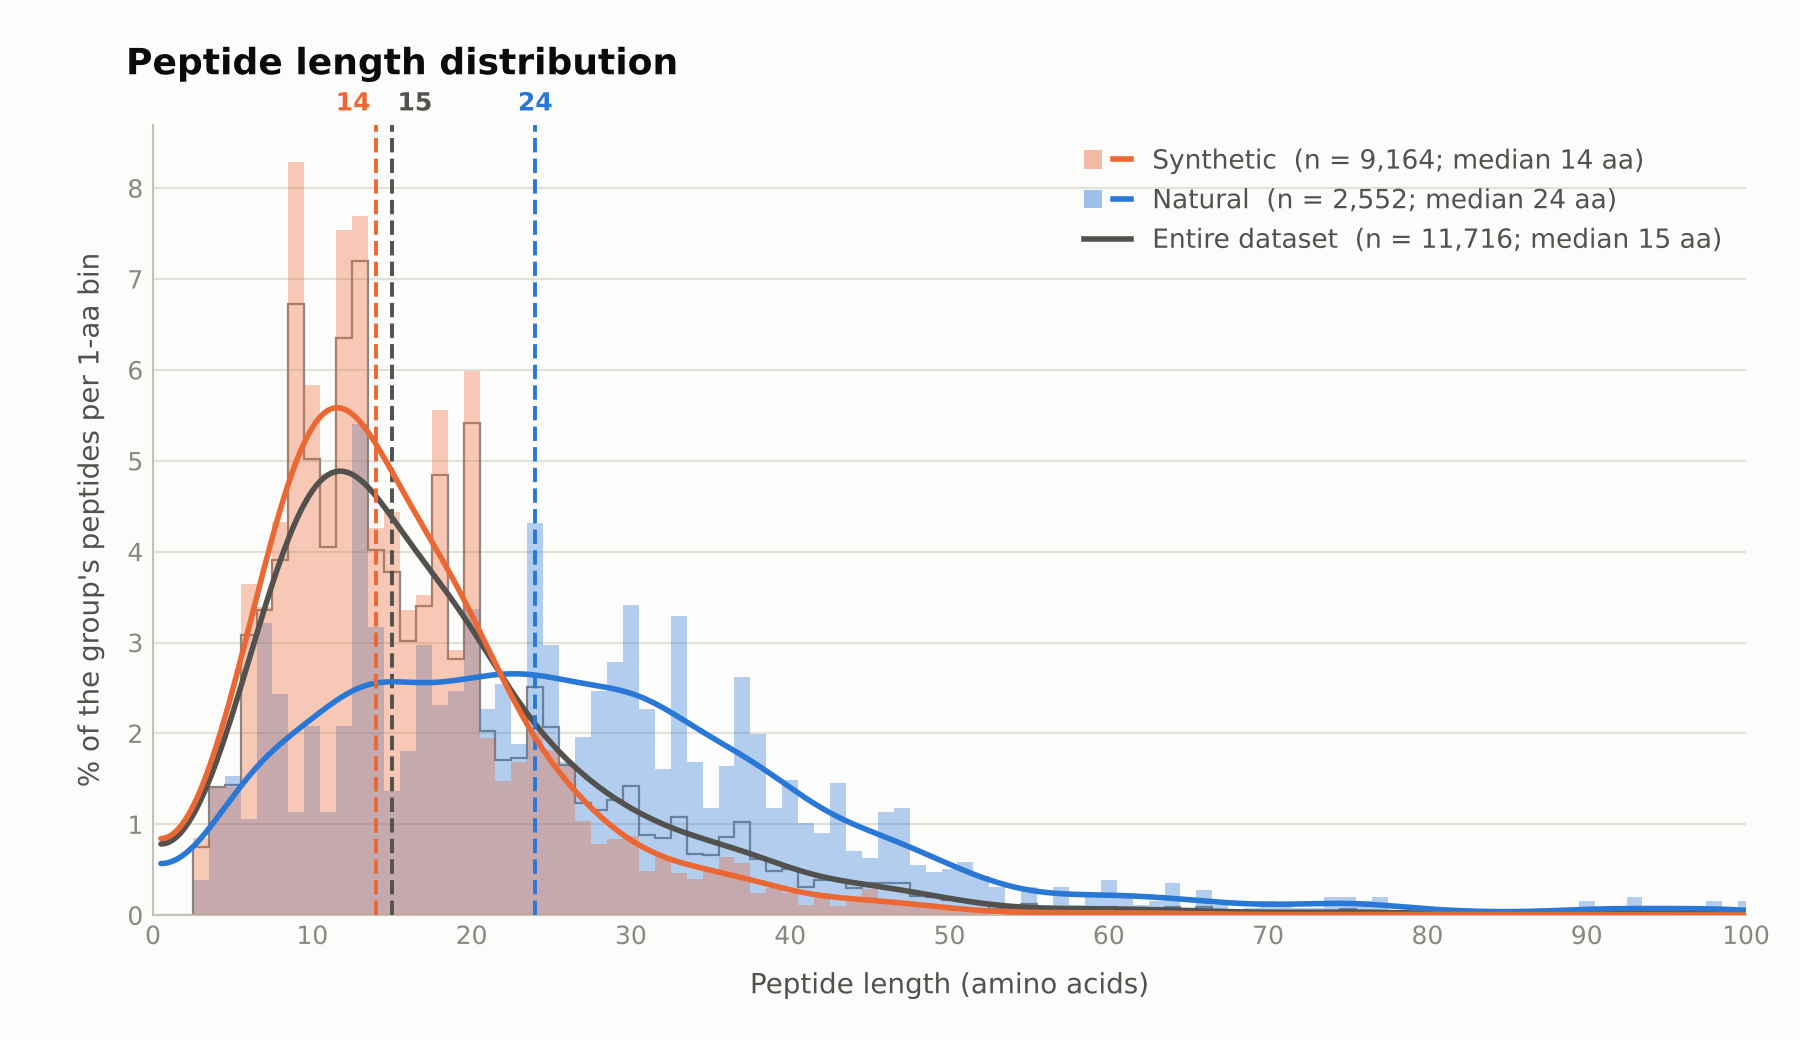
\includegraphics[width=0.86\textwidth]{deliverables/figures/length_histogram_overlap.png}
\caption{Length distribution of natural and synthetic peptides, each scaled to 100\,\% of its group. Dashed lines mark medians; curves are Gaussian kernel density estimates (bandwidth 3 residues).}
\label{fig:len}
\end{figure}

\subsection{Synthetic peptides exaggerate the cationic AMP signature; natural peptides are Cys- and Gly-rich}
Against SwissProt, both groups were enriched in Lys, Arg and Trp and depleted in Asp, Glu, Met, Gln, Thr and Ser (Fig.~\ref{fig:enr}). The synthetic profile was more extreme:
Trp $+4.17$, Lys $+1.74$, Arg $+1.20$, compared with Trp $+0.47$, Lys $+0.63$ and Arg $+0.04$ for natural peptides. Natural peptides were characterised by Cys ($+3.49$) and Gly ($+0.56$),
whereas synthetic peptides had little excess Cys ($+0.33$) and were depleted in Gly ($-0.16$). Gly and Pro changed in opposite directions in the two groups.
The non-AMP background was itself rich in Lys and Arg (10.2\,\% and 10.1\,\% of residues, vs 6.0\,\% and 5.5\,\% in SwissProt). Against it, natural peptides were depleted in Arg ($-0.44$) and unchanged in Lys,
and only synthetic peptides retained a Lys excess ($+0.61$). Trp in synthetic peptides ($+3.35$), Cys ($+1.85$) and Gly ($+1.00$) in natural peptides and depleted Met in both remained distinctive.

\begin{figure}[H]\centering
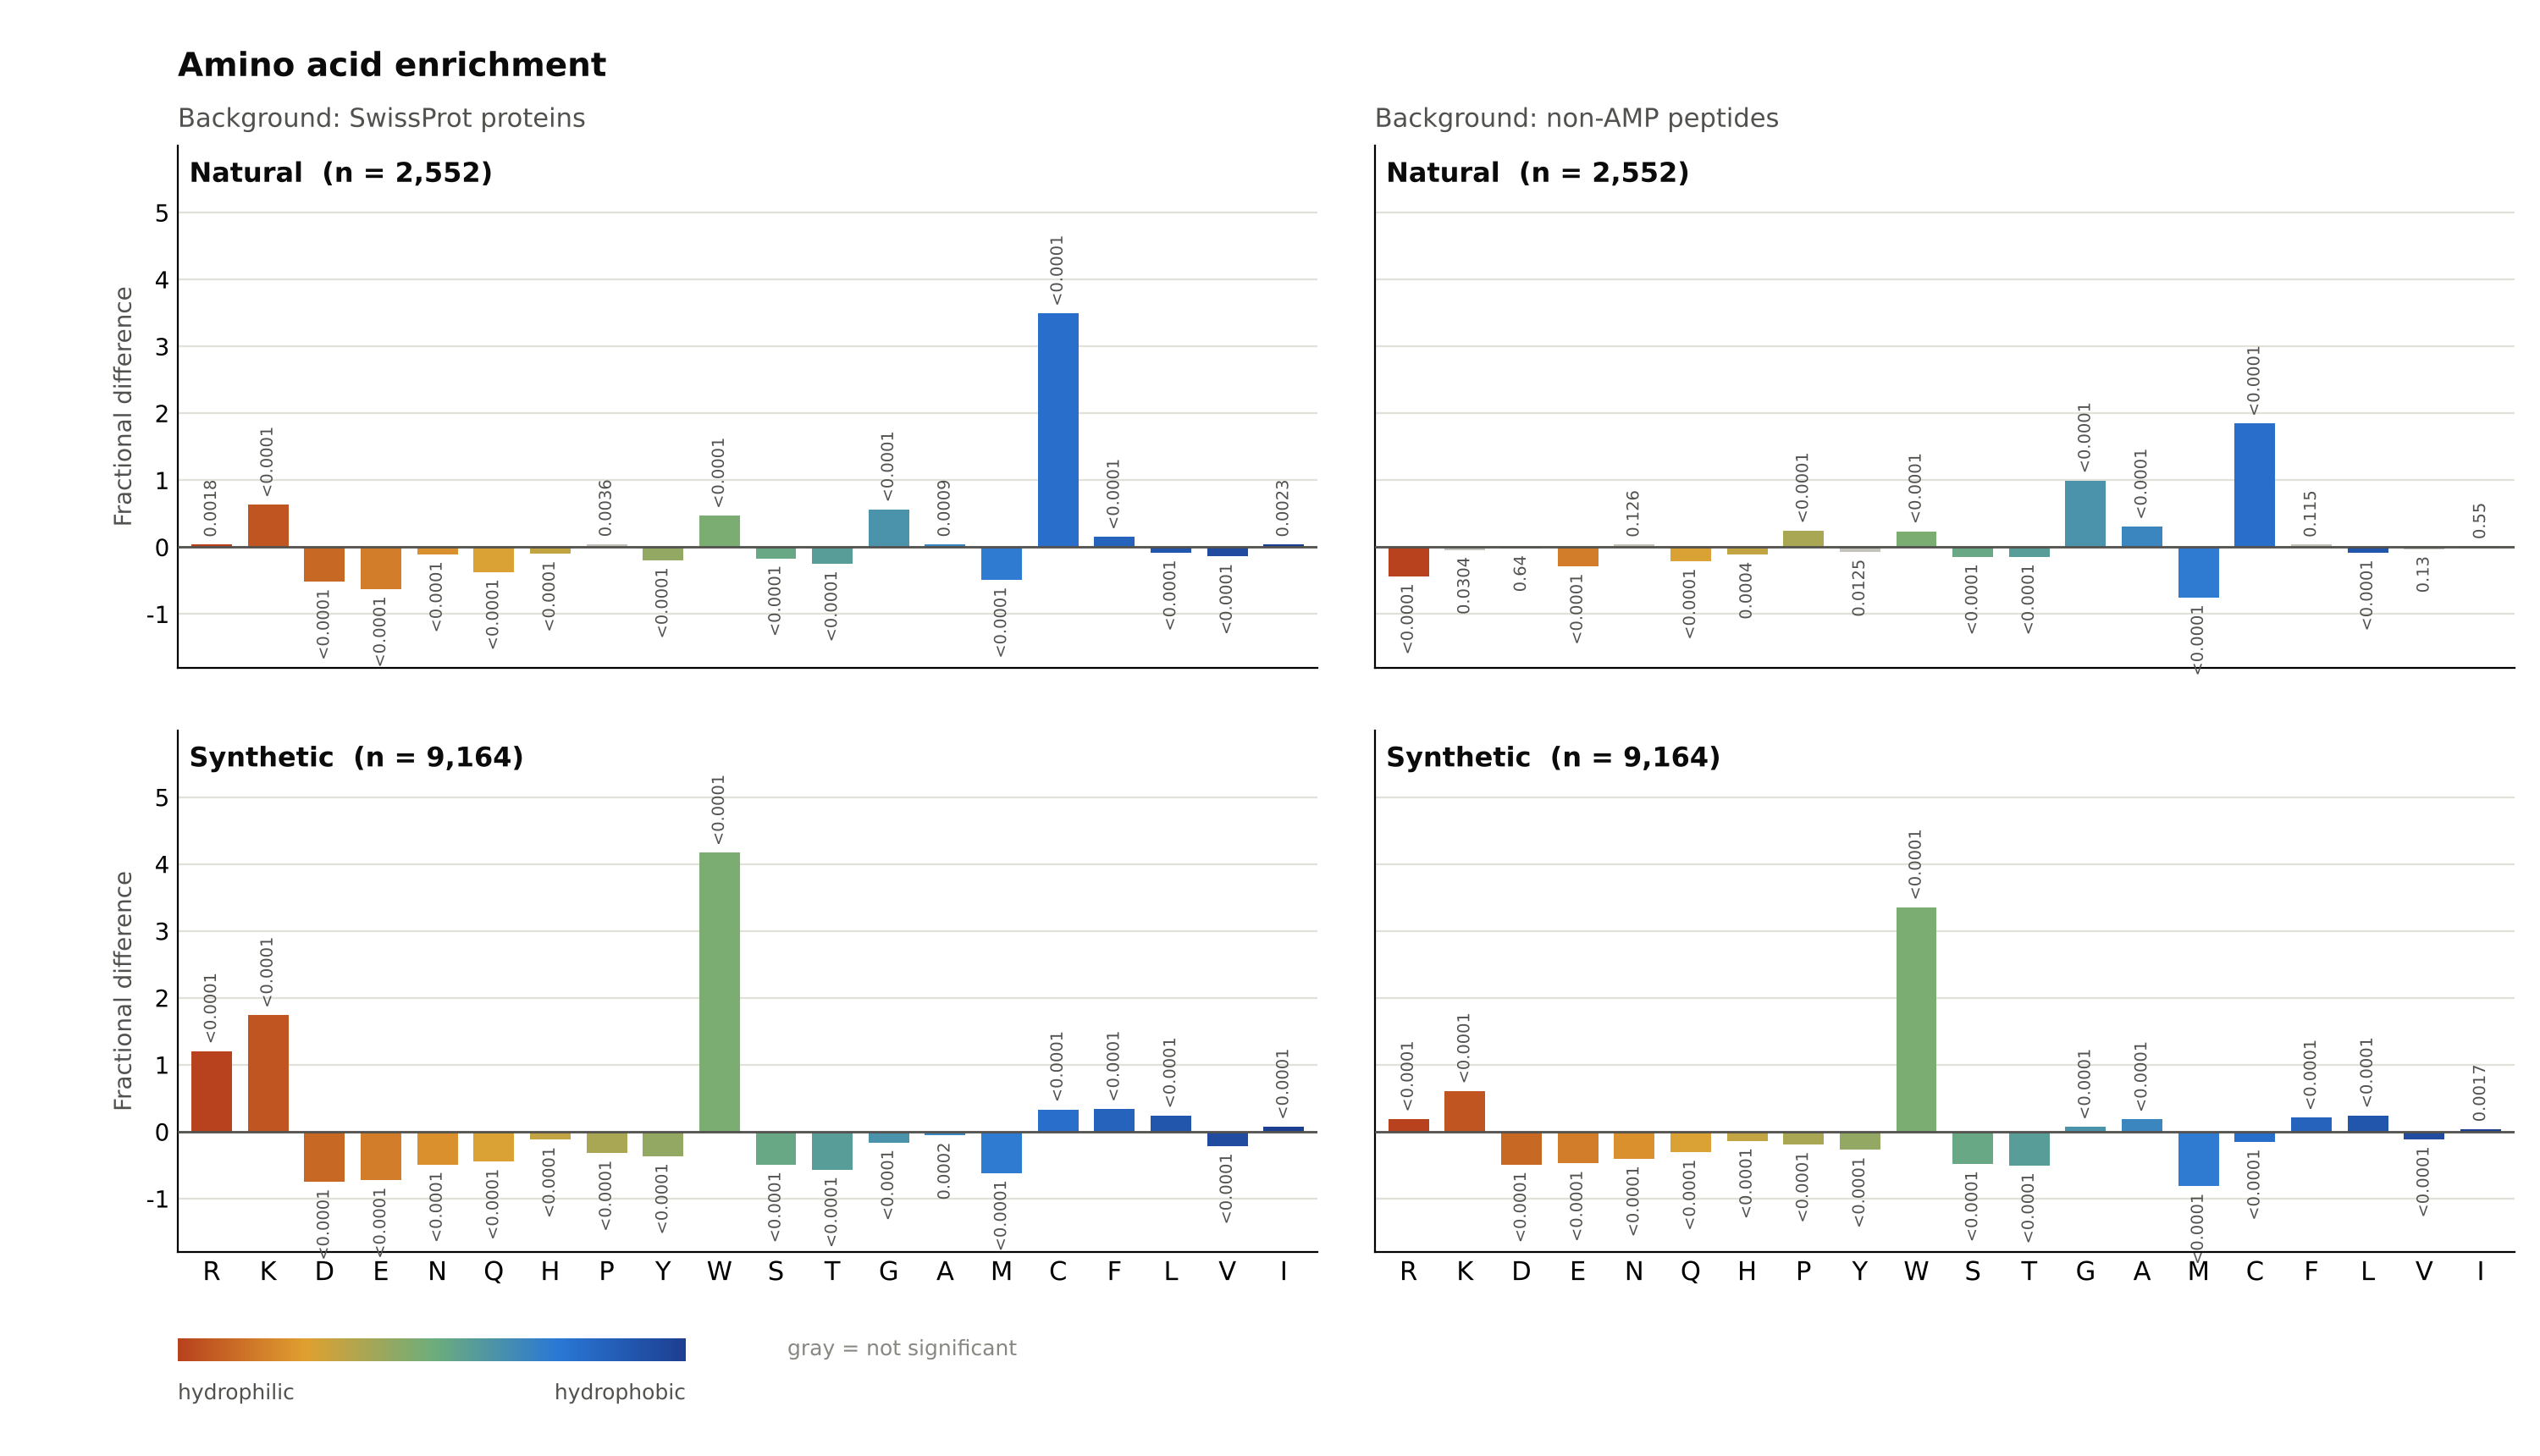
\includegraphics[width=\textwidth]{deliverables/figures/amino_acid_enrichment.png}
\caption{Amino acid enrichment of natural (top) and synthetic (bottom) peptides against SwissProt proteins (left) and non-antimicrobial peptides (right). Bars show the fractional difference; numbers are permutation p-values; grey bars are not significant after Bonferroni correction. Amino acids are ordered from hydrophilic to hydrophobic.}
\label{fig:enr}
\end{figure}

\subsection{Composition differs strongly by source organism and biosynthetic route}
All four tested kingdoms shared a natural signature---enriched Cys and Gly, depleted Met, Glu and Gln---differing mainly in degree (Fig.~\ref{fig:src}, Table~\ref{tab:src}).
Plant and fungal peptides were the most Cys-rich (Cys $+937$\,\% and $+616$\,\% vs SwissProt; $+557$\,\% and $+354$\,\% vs non-AMP). Bacterial peptides were also enriched in Trp ($+199$\,\%) and Gly and depleted in Arg;
plant peptides were depleted in hydrophobic residues (Leu, Ala, Ile, Val, Met). Splitting natural peptides by synthesis type showed that the natural signature belongs to ribosomal peptides (Cys $+361$\,\%),
whereas nonribosomal peptides formed a distinct class enriched in Pro ($+131$\,\%), Trp ($+181$\,\%), Phe and Val and depleted in Arg ($-87$\,\%), Lys, Met and Cys.
Against non-AMP peptides none of the natural classes was cationic: Arg was depleted in all four kingdoms.

\begin{figure}[H]\centering
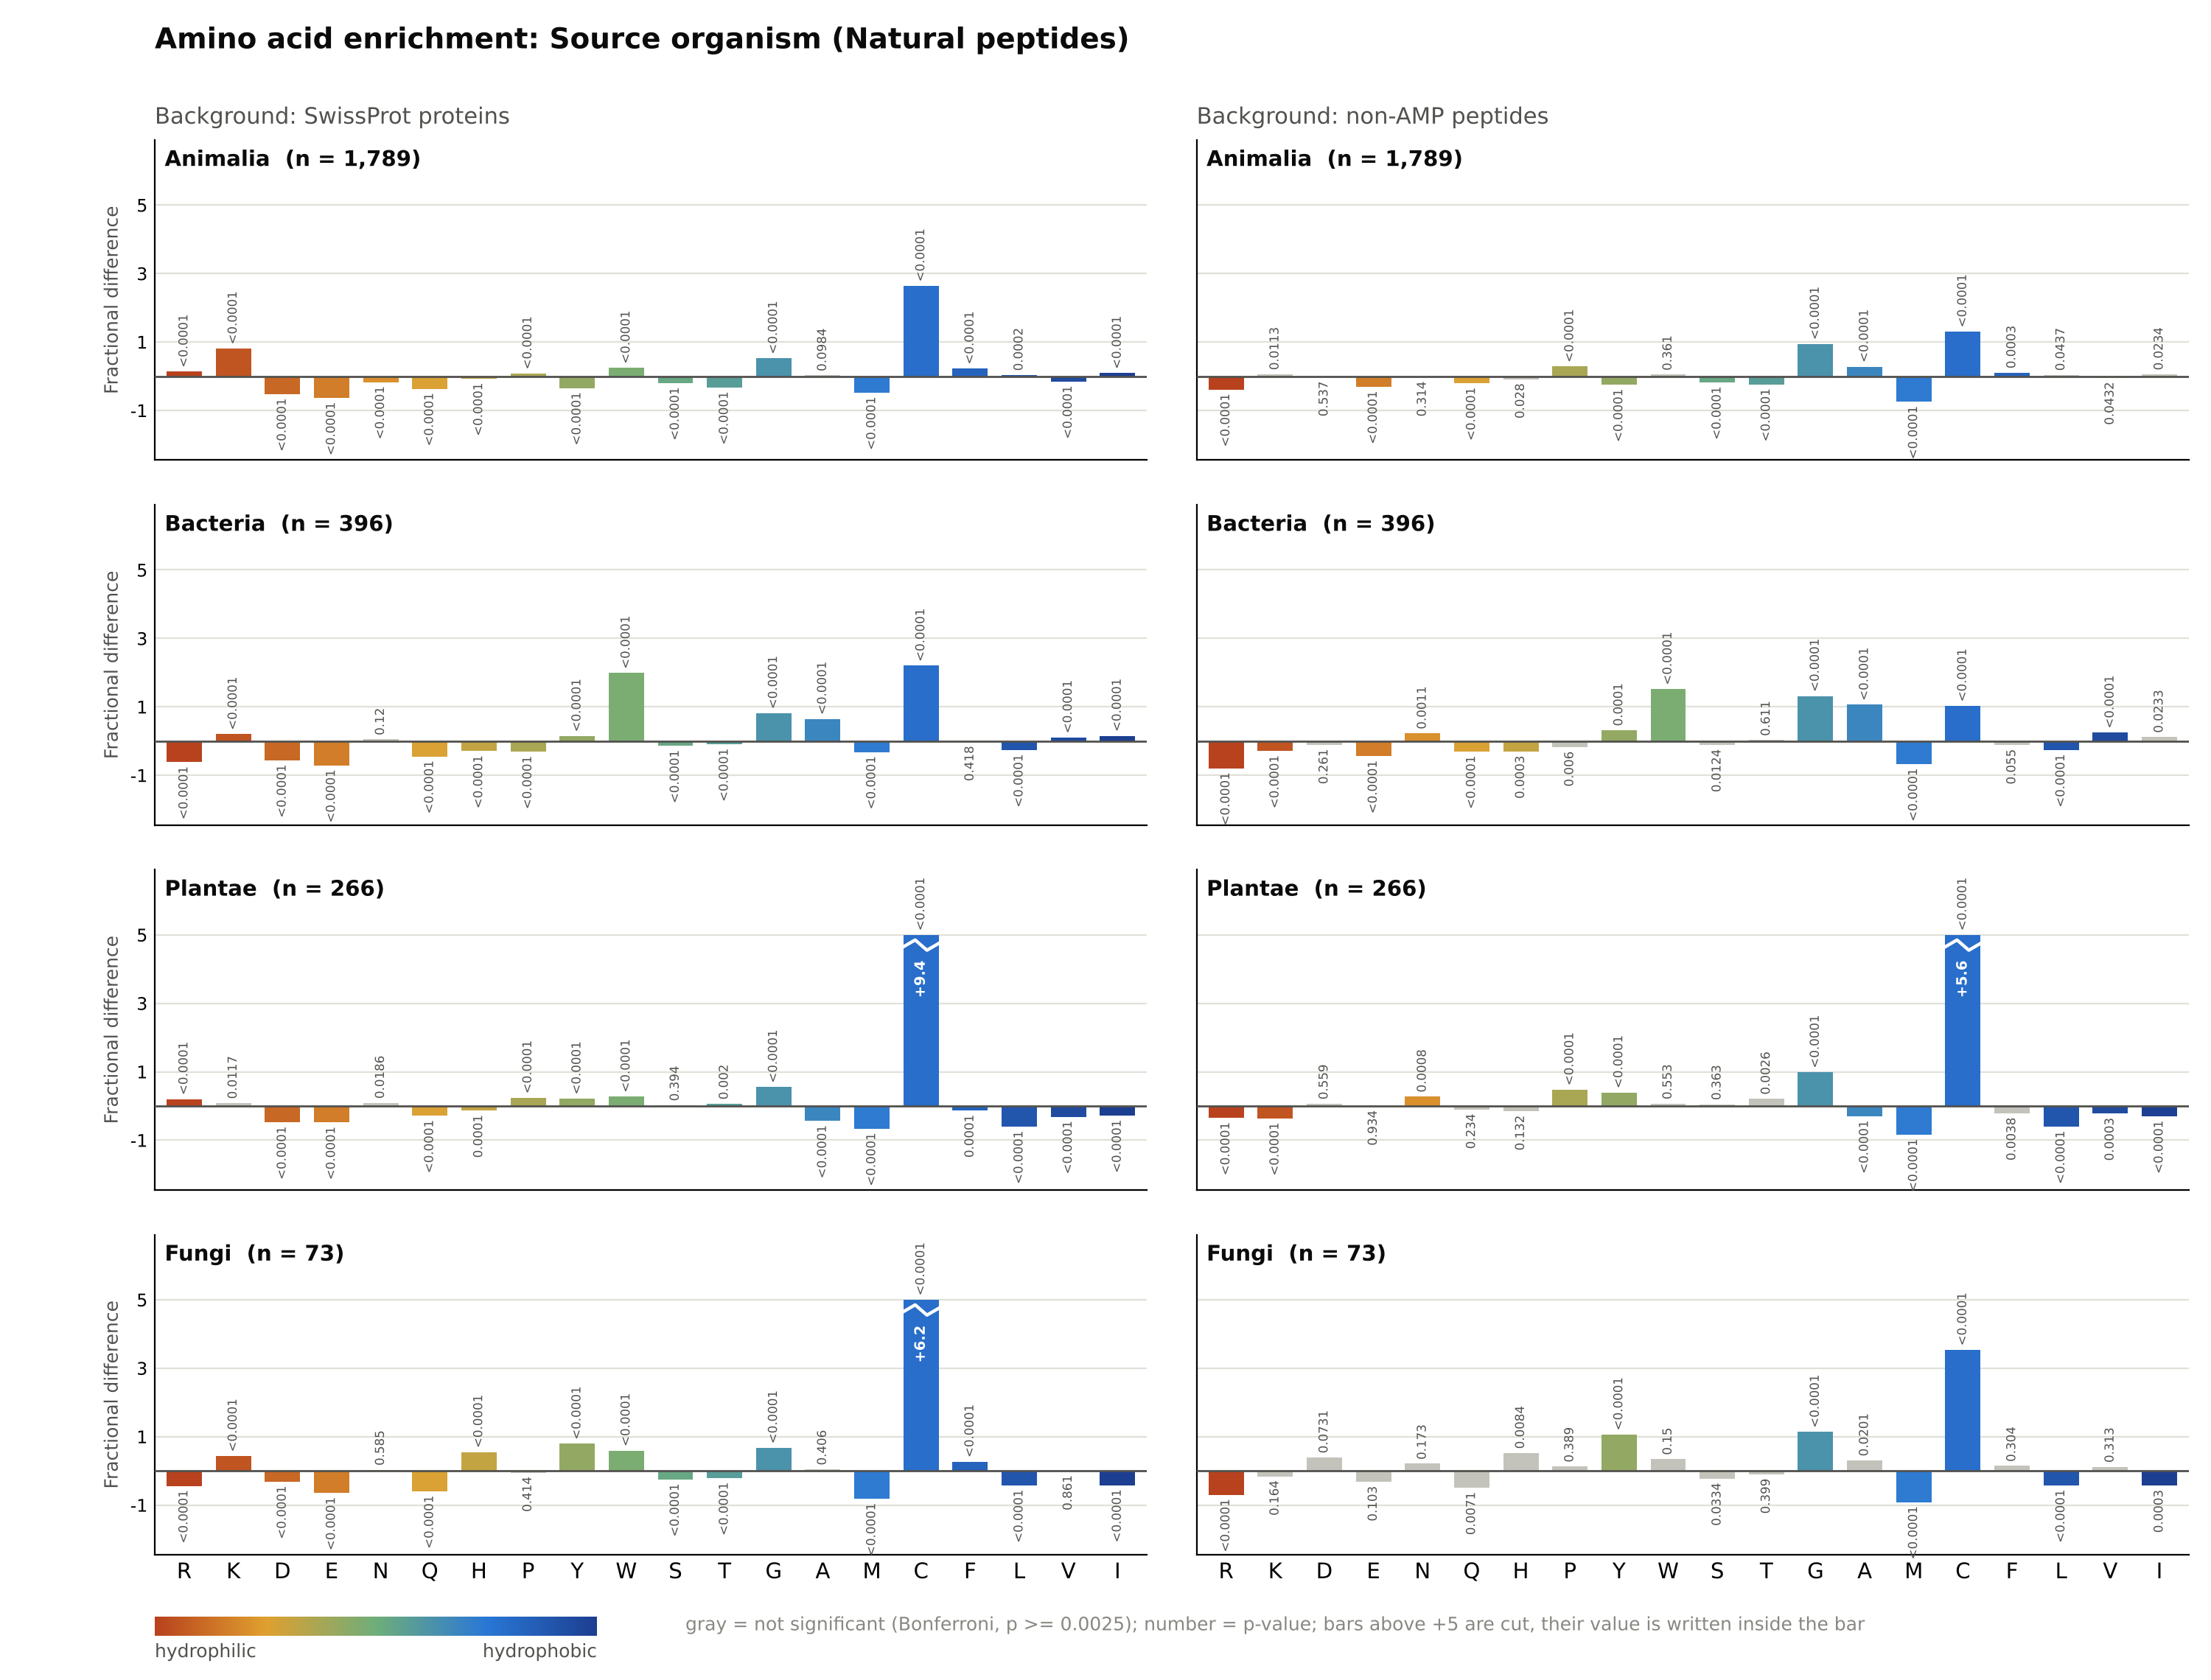
\includegraphics[width=\textwidth]{class_comparisons/source_organism/figures/amino_acid_enrichment.png}
\caption{Amino acid enrichment of natural peptides by source organism. Bars above $+5$ are cut and their value is written inside the bar. Layout as in Fig.~\ref{fig:enr}.}
\label{fig:src}
\end{figure}

\begin{table}[H]\centering\small
\begin{tabular}{lrrrrrrrr}
\toprule
Class ($n$) & median aa & C & G & W & K & R & P & M\\\midrule
Animalia (1{,}789) & 24 & 264 & 52 & 24 & 81 & 13 & 8 & $-48$\\
Bacteria (396) & 18 & 220 & 82 & 199 & 20 & $-62$ & $-31$ & $-32$\\
Plantae (266) & 30.5 & 937 & 55 & 27 & 9$^{\text{ns}}$ & 20 & 24 & $-66$\\
Fungi (73) & 6 & 616 & 67 & 60 & 43 & $-44$ & $-5^{\text{ns}}$ & $-82$\\
Ribosomal (2{,}301) & 26 & 361 & 59 & 43 & 67 & 7 & $1^{\text{ns}}$ & $-48$\\
Nonribosomal (251) & 7 & $-51$ & $-51$ & 181 & $-60$ & $-87$ & 131 & $-87$\\
Synthetic (9{,}164) & 14 & 33 & $-16$ & 417 & 174 & 121 & $-32$ & $-62$\\\bottomrule
\end{tabular}
\caption{Median length and percentage change versus SwissProt for selected amino acids (ns: not significant; all other values $p < 0.0025$).}
\label{tab:src}
\end{table}

\subsection{Target groups share the composition of their source}
Target groups overlapped extensively (median three labels per peptide; Jaccard index 0.83 between the anti-Gram-positive and anti-Gram-negative classes). With all peptides, every target group showed the synthetic profile
(Trp, Lys and Cys up; Glu, Asp, Met, Thr and Gln down), except antiviral peptides, in which Glu and Gln were not depleted. Restricted to natural peptides, the target groups largely shared the natural signature
(Cys $+88$ to $+531$\,\%, Gly $+38$ to $+58$\,\%; Fig.~\ref{fig:fun}). Residual differences were modest: peptides tested on mammalian cells were additionally enriched in Lys and Trp, anticancer peptides in Pro, Phe and Ile,
and the small antibiofilm class ($n=53$) showed the weakest Cys signal. Anticancer natural peptides were also shorter than other natural peptides (median 18.5 vs 25 residues, $r=-0.30$).

\begin{figure}[H]\centering
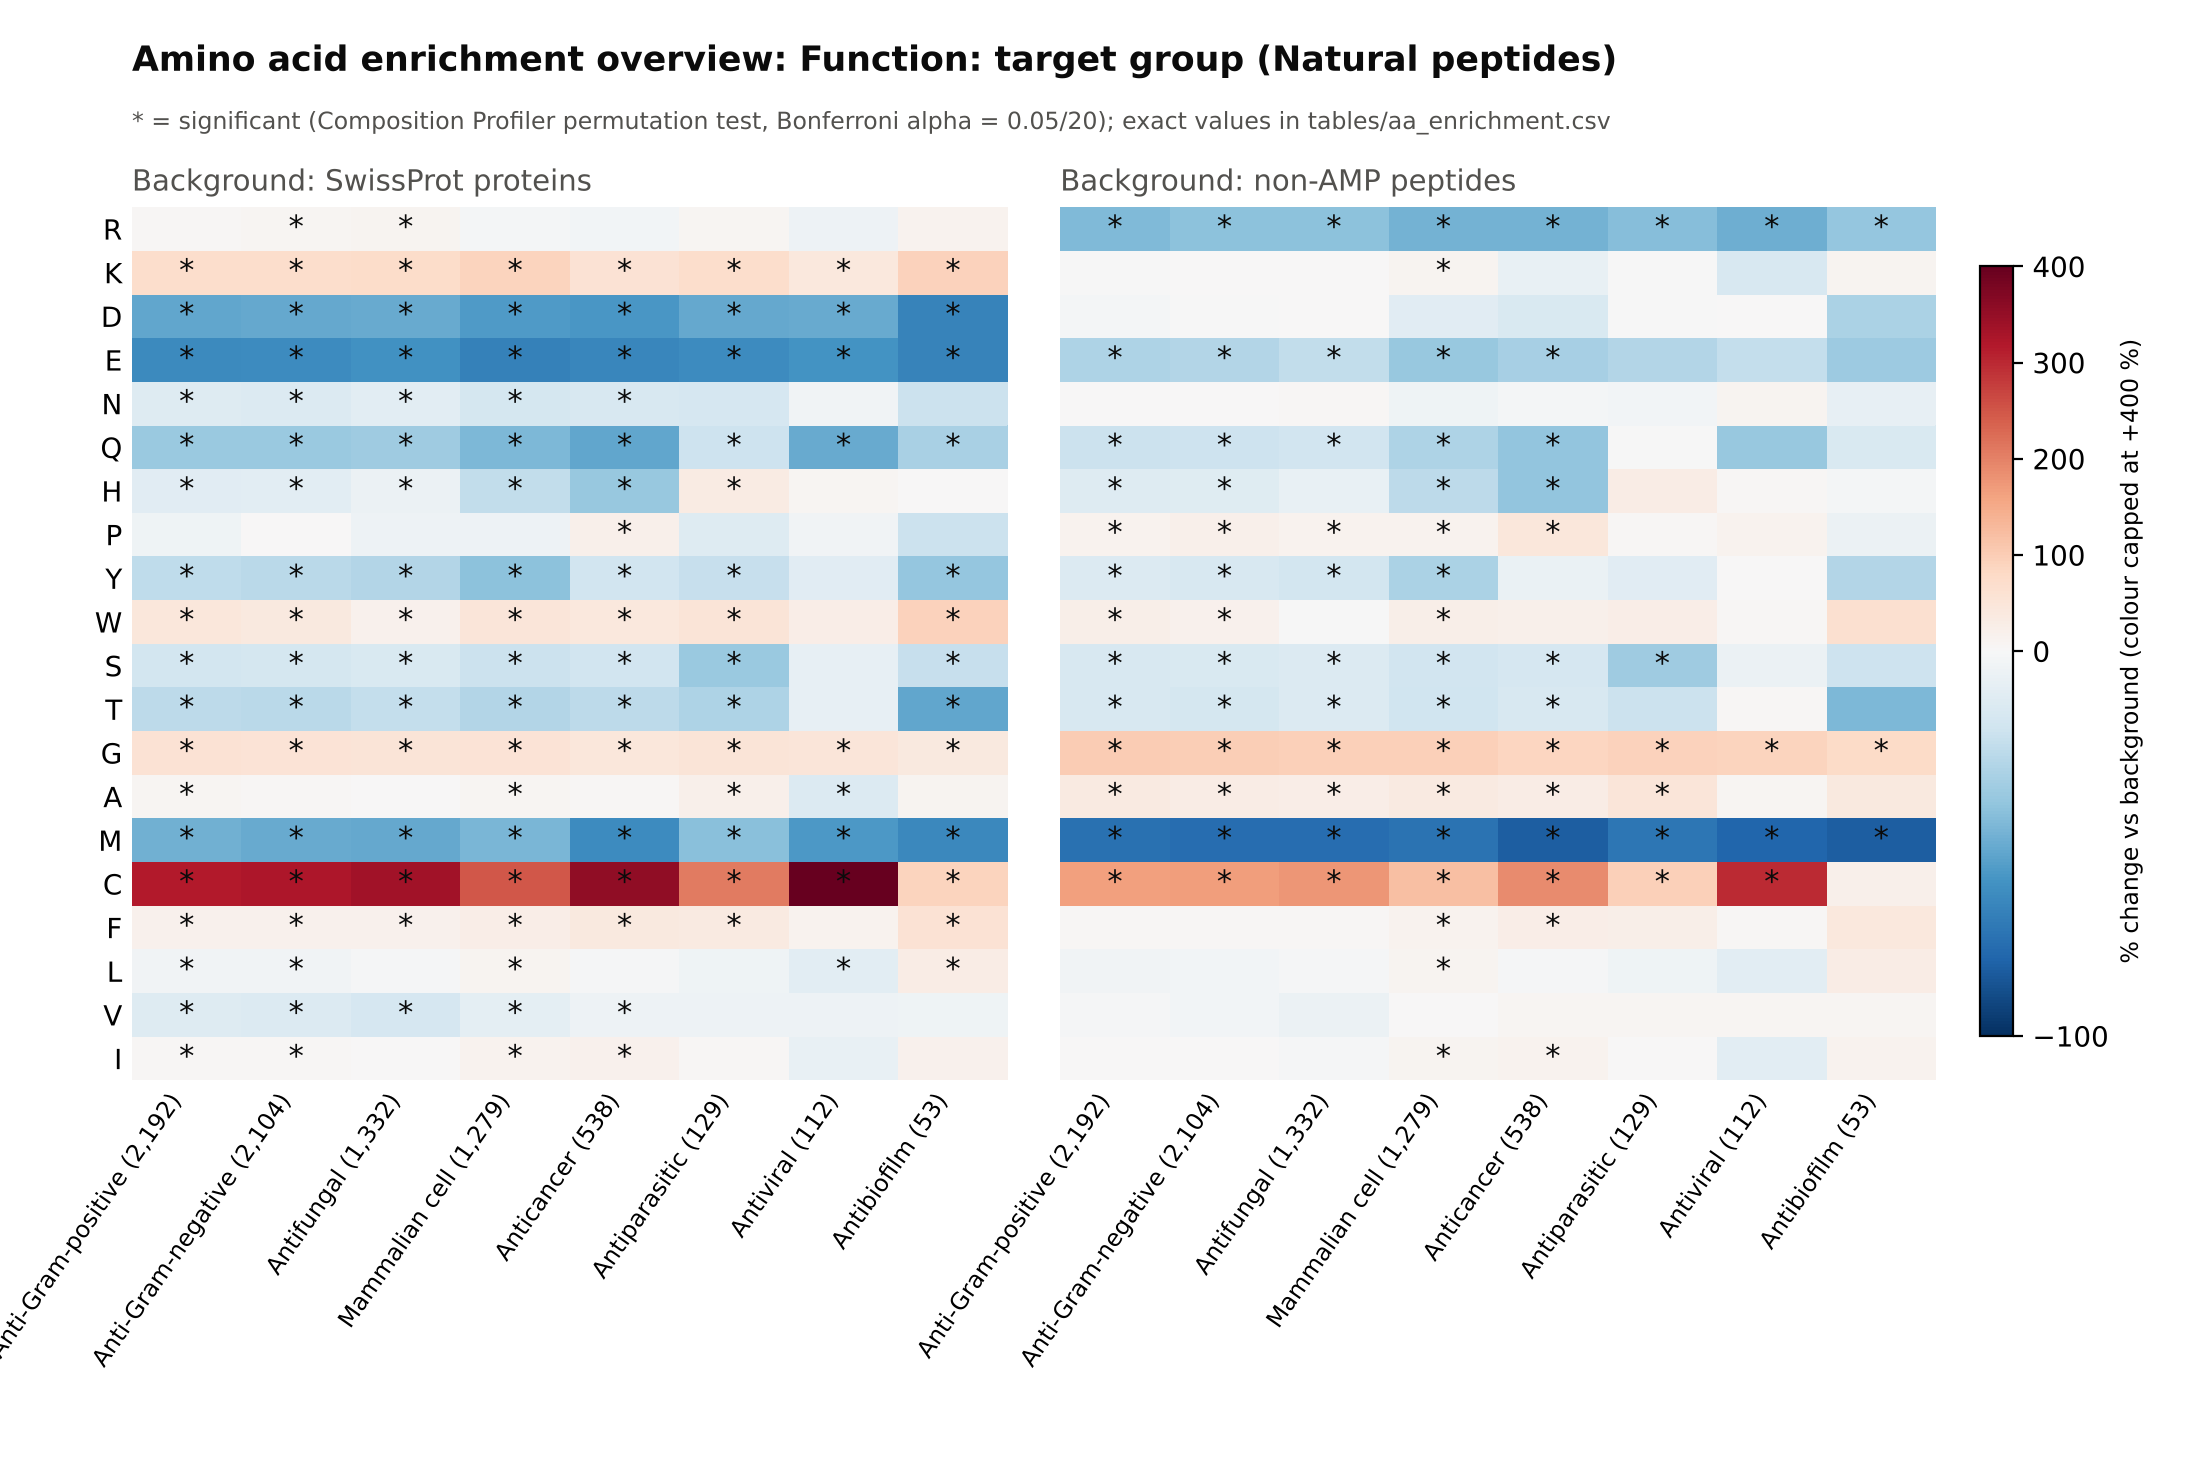
\includegraphics[width=0.95\textwidth]{class_comparisons/function_natural/figures/enrichment_heatmap.png}
\caption{Amino acid enrichment of natural peptides by target group (\% change; asterisks mark significance after Bonferroni correction).}
\label{fig:fun}
\end{figure}

\subsection{Target object separates distinct peptide families}
In contrast to target group, target object separated classes with distinct compositions (Fig.~\ref{fig:to}). Peptides acting on the ribosome ($n=59$) or on cytoplasmic proteins ($n=176$) were enriched in Pro
($+625$\,\% and $+303$\,\%) and Arg ($+333$\,\% and $+237$\,\%) and lacked Cys entirely in the ribosome class. Lipid II binders ($n=81$) were enriched in Cys ($+514$\,\%), Thr and Ile and depleted in Arg and Pro.
Virus-entry peptides ($n=342$) were enriched in Trp ($+265$\,\%) but also in Glu ($+34$\,\%) and Gln ($+37$\,\%), and depleted in Pro; they were the longest class (median 21 residues, $r=+0.41$).
Virus-integrase peptides were short (median 11) and Trp-rich ($+543$\,\%), DNA/RNA-binding peptides were cationic and Trp-rich, and lipid-bilayer peptides, 82\,\% of the dataset, reproduced the overall AMP pattern.

\begin{figure}[H]\centering
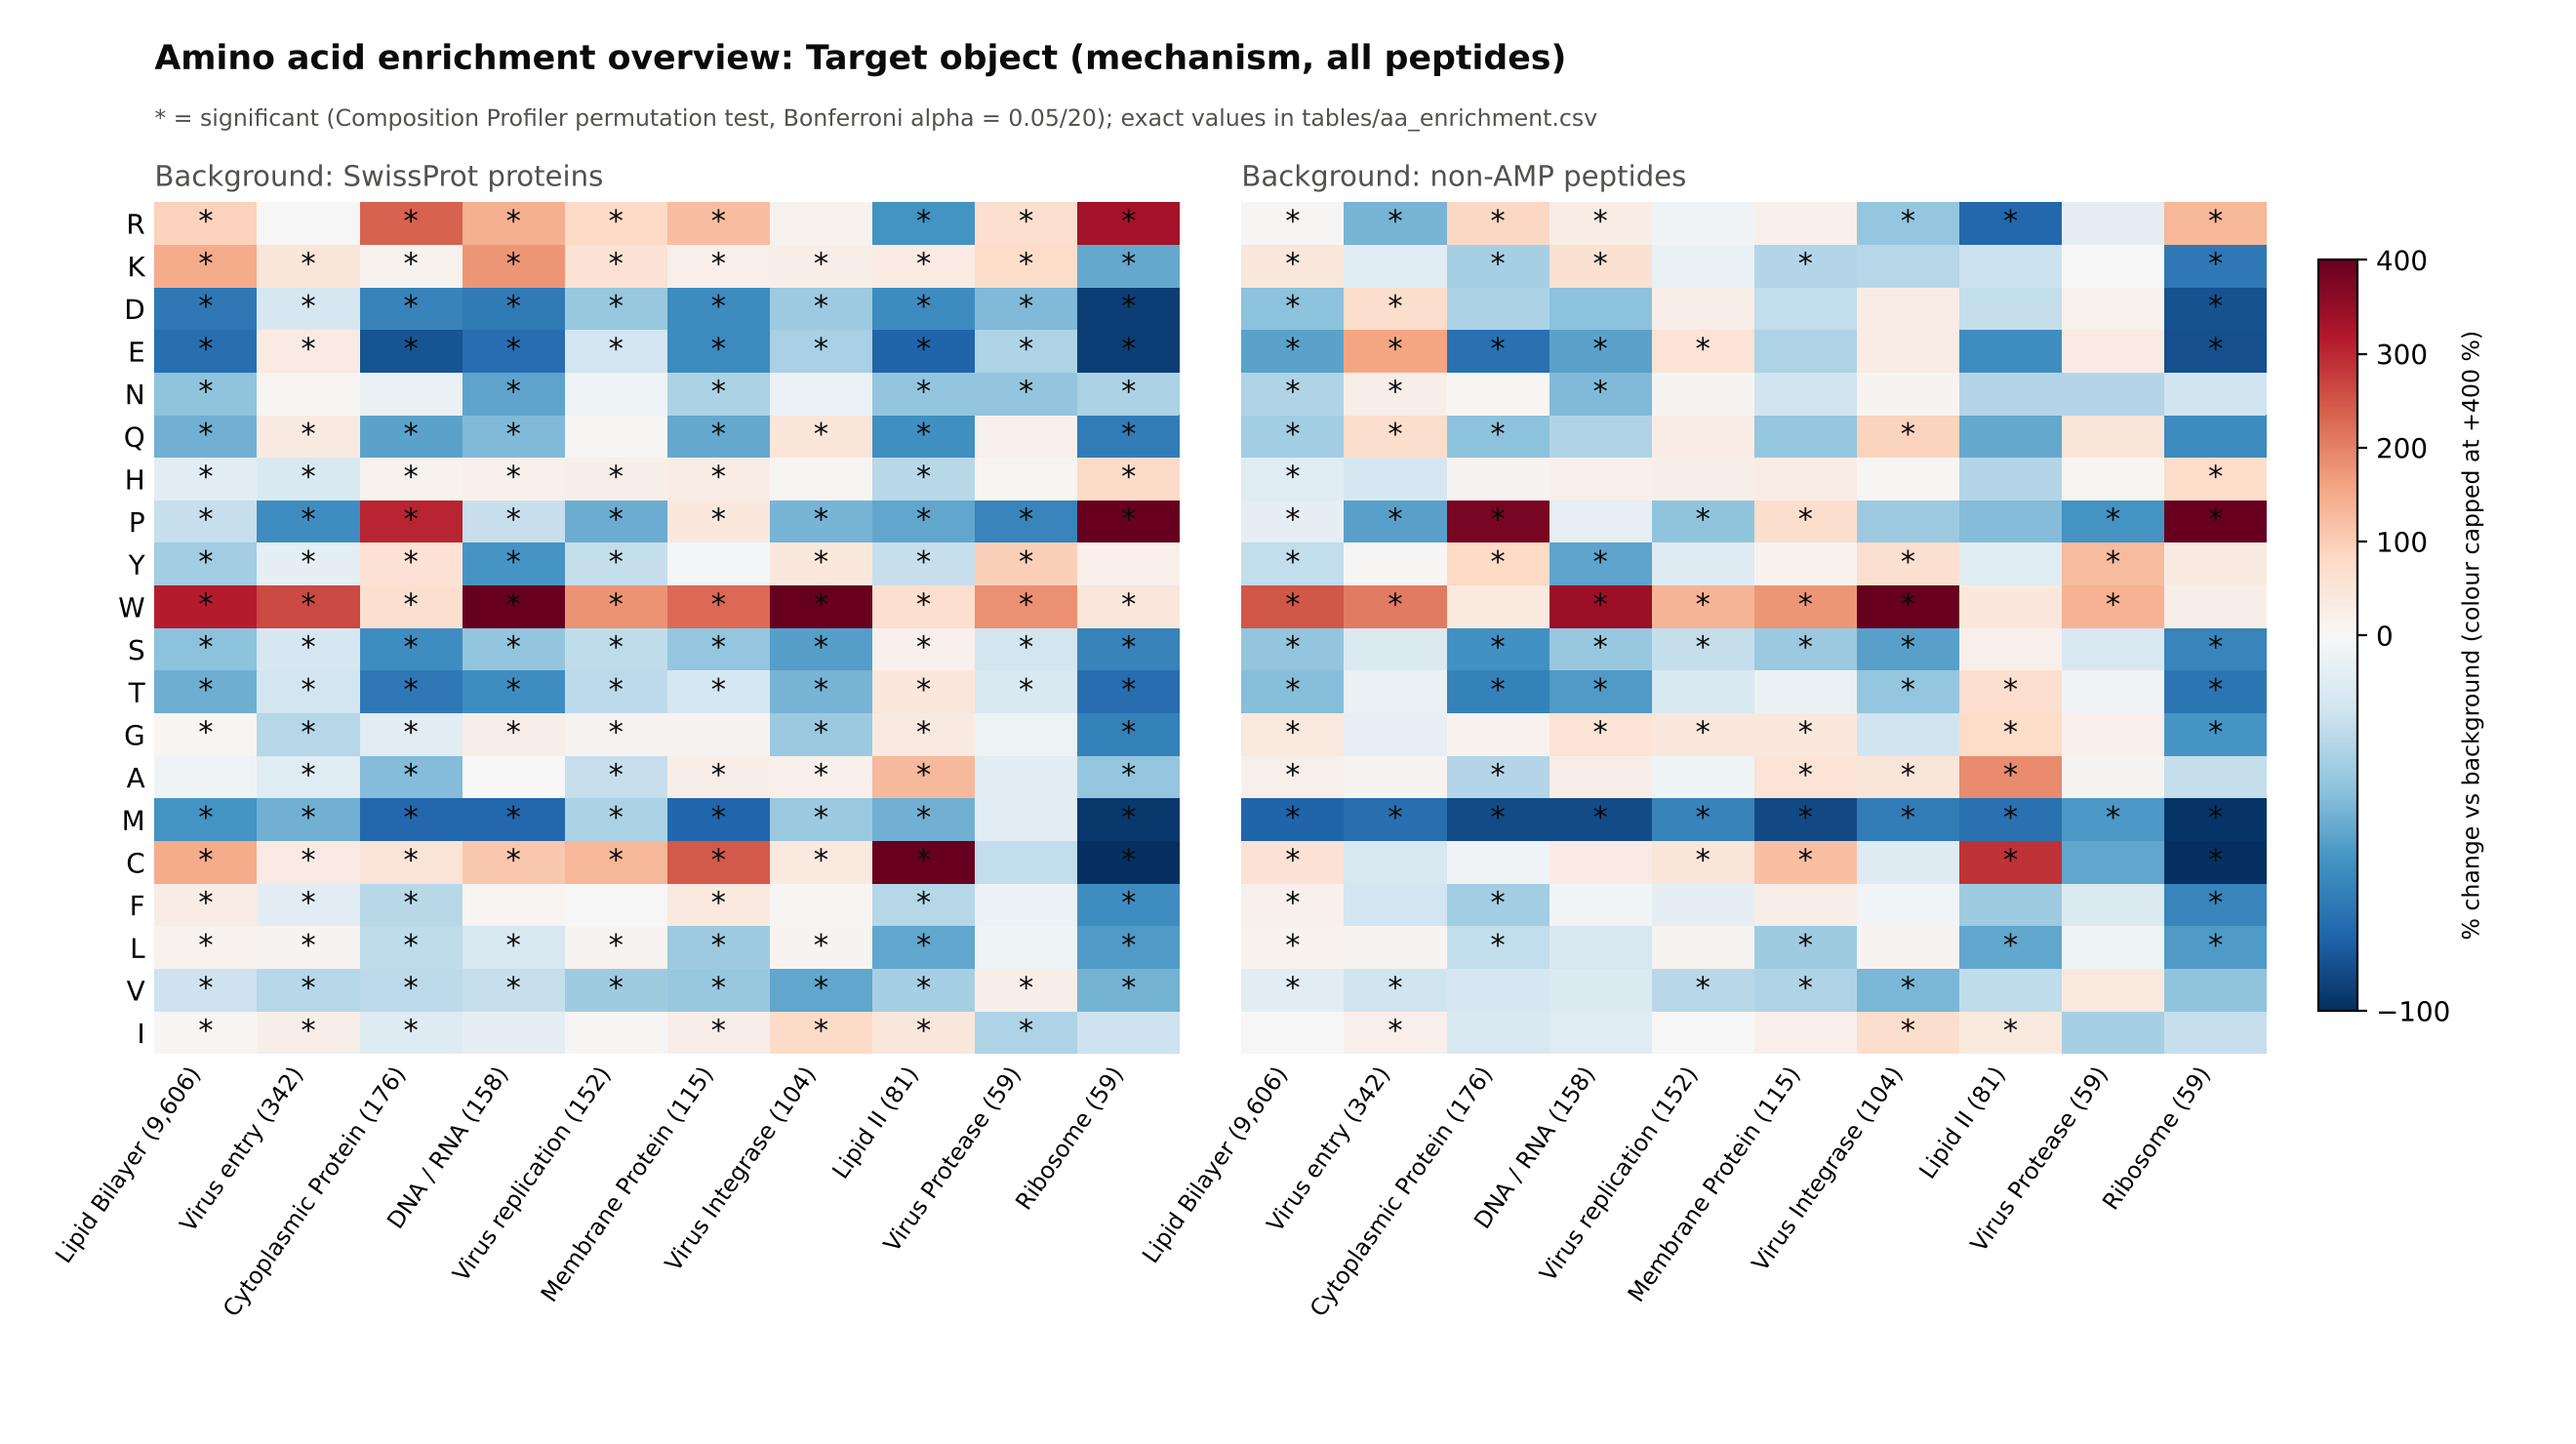
\includegraphics[width=\textwidth]{class_comparisons/target_object/figures/enrichment_heatmap.png}
\caption{Amino acid enrichment by target object (\% change, colour capped at $+400$\,\%; asterisks mark significance after Bonferroni correction).}
\label{fig:to}
\end{figure}

\subsection{Length varies with source and mechanism}
Median lengths differed across kingdoms (plants 30.5, animals 24, bacteria 18, fungi 6 residues; Kruskal--Wallis $p = 10^{-36}$) and synthesis types (ribosomal 26, synthetic 14, nonribosomal 7; $p<10^{-300}$; Fig.~\ref{fig:box}).
71\,\% of fungal and 70\,\% of nonribosomal peptides were 3--9 residues long. Across target groups medians lay between 13 and 18 residues for all peptides, whereas target objects ranged from 11 (virus integrase, Lipid II) to 21 (virus entry).

\begin{figure}[H]\centering
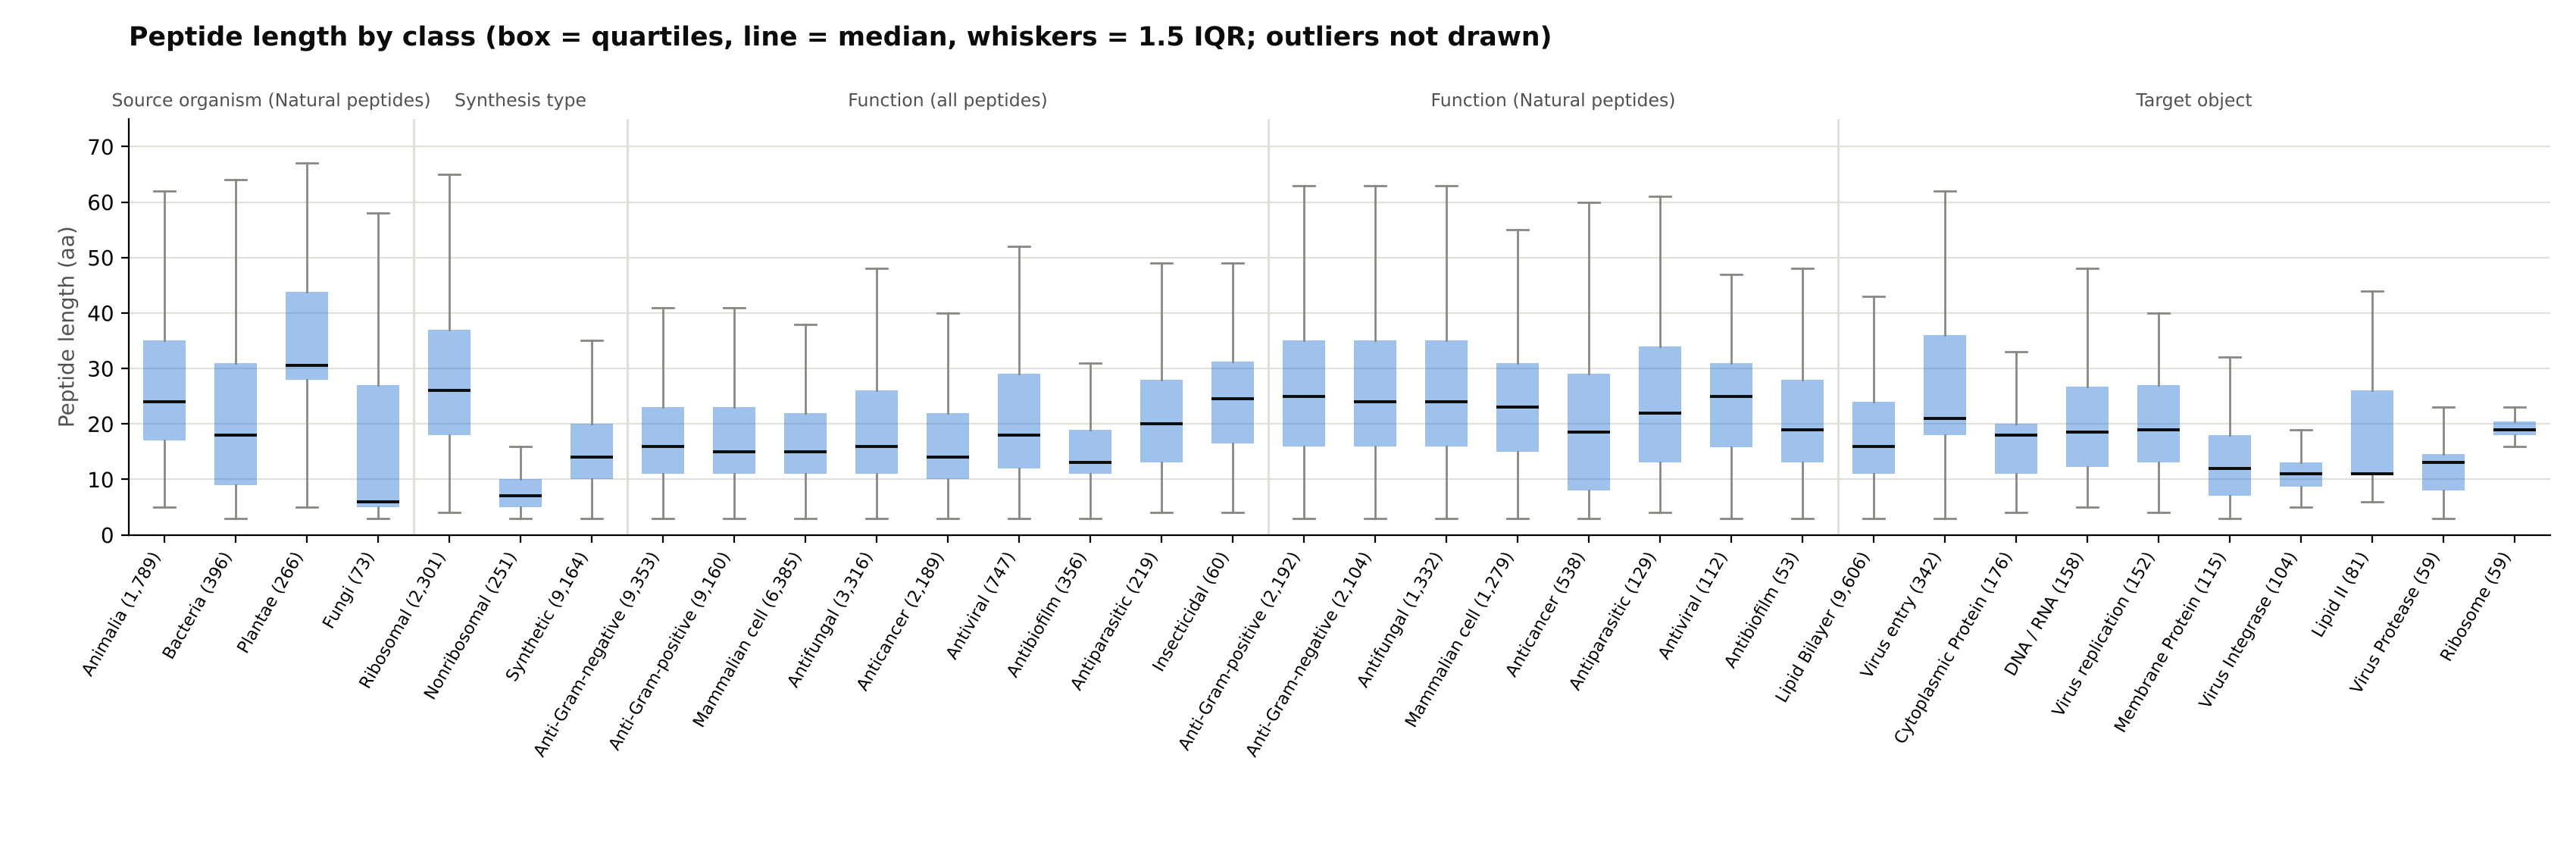
\includegraphics[width=\textwidth]{class_comparisons/overview/figures/length_boxplots.png}
\caption{Length of every tested class (boxes: quartiles; lines: medians; whiskers: 1.5 interquartile range; outliers not shown).}
\label{fig:box}
\end{figure}

%=====================================================================
\section{Discussion}
%=====================================================================
After removing near-duplicate sequences, natural and synthetic AMPs in DBAASP differ systematically. Synthetic peptides occupy a narrow region of sequence space: short, strongly cationic and Trp-rich,
with little Cys---the footprint of rational design, in which positive charge and Trp/Arg motifs are increased to enhance membrane binding \cite{chan2006} and length is kept short to reduce synthesis cost.
The high redundancy of synthetic entries shows that much of the synthetic data consists of analogue series.

Natural AMPs are longer and are distinguished above all by Cys and Gly, reflecting disulfide-stabilised families such as defensins \cite{ganz2003}, especially in plants and fungi, where Cys is seven- to ten-fold
enriched relative to ordinary proteins. Nonribosomal peptides diverge from both groups: short, rich in Pro and aromatic residues and poor in basic residues, with frequent D-amino acids (52\,\%) and N-terminal modifications (37\,\%).

The second background changes the interpretation of the cationic signature. Relative to proteins, all AMP classes are Lys/Arg-rich; relative to non-antimicrobial peptides that are themselves Lys/Arg-rich, natural AMPs are not.
Charge alone is therefore shared with many short bioactive peptides, whereas Trp, Cys/Gly and the depletion of Met distinguish AMPs from other peptides of similar length. Because the non-AMP set was not audited here,
this conclusion should be checked against an independently curated, length-matched negative set.

Within natural peptides, target group explained little compositional variation once source was taken into account. Target labels in DBAASP indicate that activity was measured against a target, not that the peptide is potent,
and most peptides are tested against several targets. Mechanism, by contrast, identified well-known families: the Pro/Arg-rich, Cys-free composition of ribosome- and cytoplasmic-protein-targeting peptides matches the proline-rich AMPs
that enter bacteria and bind the ribosome exit tunnel \cite{graf2017}; the Cys/Thr-rich Lipid II class is consistent with lantibiotics and defensin-like Lipid II binders \cite{breukink2006}; and the Glu/Gln-rich, Pro-poor
virus-entry class is consistent with peptides derived from viral fusion proteins. Composition-based classifiers might therefore predict mechanism better than tested activity.

\paragraph{Limitations.}
(i) Kingdom is available only for natural peptides. (ii) The SwissProt background is an older sample of 5{,}002 proteins, and the non-AMP background was used as supplied.
(iii) Replacement of \texttt{X} by alanine inflates alanine, slightly overall (0.65\,\% of natural and 1.17\,\% of synthetic residues) but strongly in nonribosomal (10.4\,\%) and Lipid II peptides (9.9\,\%), whose alanine results we do not interpret.
(iv) Residue frequencies were pooled without length adjustment, and D-amino acids and terminal modifications were not considered. (v) Target groups and objects overlap, several classes are small (fungi $n=73$; ribosome $n=59$),
and all associations are descriptive.

%=====================================================================
\section{Conclusions}
%=====================================================================
A redundancy-reduced survey of the complete DBAASP peptide list shows that biosynthetic origin, source organism and mechanism shape AMP length and composition more than the activities a peptide was tested for.
Synthetic AMPs are short and Trp/Lys/Arg-rich; natural ribosomal AMPs are longer and Cys/Gly-rich, most strongly in plants and fungi; nonribosomal peptides form a separate Pro- and aromatic-rich class;
and intracellular, Lipid II-binding and virus-entry peptides each have their own signature. Models trained on database entries without redundancy control or class stratification will mainly learn the synthetic design pattern.

\section*{Data availability}
The cleaned dataset (11{,}716 sequences in FASTA format), per-class FASTA files, all intermediate tables, the record-level loss table and the analysis scripts are available at \todo{repository URL / DOI}.

\section*{Author contributions}
\todo{To be completed.}

\section*{Competing interests}
\todo{To be completed.}

\begin{thebibliography}{99}\small
\bibitem{zasloff2002} Zasloff M. Antimicrobial peptides of multicellular organisms. \emph{Nature}. 2002;415:389--395. doi:10.1038/415389a
\bibitem{hancock2006} Hancock REW, Sahl HG. Antimicrobial and host-defense peptides as new anti-infective therapeutic strategies. \emph{Nat Biotechnol}. 2006;24:1551--1557. doi:10.1038/nbt1267
\bibitem{ganz2003} Ganz T. Defensins: antimicrobial peptides of innate immunity. \emph{Nat Rev Immunol}. 2003;3:710--720. doi:10.1038/nri1180
\bibitem{chan2006} Chan DI, Prenner EJ, Vogel HJ. Tryptophan- and arginine-rich antimicrobial peptides: structures and mechanisms of action. \emph{Biochim Biophys Acta}. 2006;1758:1184--1202. doi:10.1016/j.bbamem.2006.04.006
\bibitem{graf2017} Graf M, Mardirossian M, Nguyen F, et al. Proline-rich antimicrobial peptides targeting protein synthesis. \emph{Nat Prod Rep}. 2017;34:702--711. doi:10.1039/c7np00020k
\bibitem{breukink2006} Breukink E, de Kruijff B. Lipid II as a target for antibiotics. \emph{Nat Rev Drug Discov}. 2006;5:321--332. doi:10.1038/nrd2004
\bibitem{pirtskhalava2021} Pirtskhalava M, Amstrong AA, Grigolava M, et al. DBAASP v3: database of antimicrobial/cytotoxic activity and structure of peptides as a resource for development of new therapeutics. \emph{Nucleic Acids Res}. 2021;49:D288--D297. doi:10.1093/nar/gkaa991
\bibitem{wang2016} Wang G, Li X, Wang Z. APD3: the antimicrobial peptide database as a tool for research and education. \emph{Nucleic Acids Res}. 2016;44:D1087--D1093. doi:10.1093/nar/gkv1278
\bibitem{wang2022} Wang G. Unifying the classification of antimicrobial peptides in the antimicrobial peptide database. \emph{Methods Enzymol}. 2022;663:1--18. doi:10.1016/bs.mie.2021.09.006
\bibitem{li2006} Li W, Godzik A. Cd-hit: a fast program for clustering and comparing large sets of protein or nucleotide sequences. \emph{Bioinformatics}. 2006;22:1658--1659. doi:10.1093/bioinformatics/btl158
\bibitem{fu2012} Fu L, Niu B, Zhu Z, Wu S, Li W. CD-HIT: accelerated for clustering the next-generation sequencing data. \emph{Bioinformatics}. 2012;28:3150--3152. doi:10.1093/bioinformatics/bts565
\bibitem{vacic2007} Vacic V, Uversky VN, Dunker AK, Lonardi S. Composition Profiler: a tool for discovery and visualization of amino acid composition differences. \emph{BMC Bioinformatics}. 2007;8:211. doi:10.1186/1471-2105-8-211
\bibitem{uniprot2023} The UniProt Consortium. UniProt: the Universal Protein Knowledgebase in 2023. \emph{Nucleic Acids Res}. 2023;51:D523--D531. doi:10.1093/nar/gkac1052
\end{thebibliography}

\end{document}
